\documentclass[12pt]{article}
\usepackage{scrextend}
\usepackage[utf8]{inputenc}
\usepackage[polish]{babel}
\usepackage[T1]{fontenc}%polskie znaki
\usepackage[utf8]{inputenc}%polskie znaki
\usepackage{geometry}
\usepackage{float}
\usepackage{enumitem}
\usepackage{hyperref}
\usepackage{graphicx}
\usepackage{tabulary}
\usepackage{etoc}
\usepackage[normalem]{ulem} 
\usepackage{tikz}
\usepackage[bf]{caption}
\usepackage{listings}
\renewcommand{\baselinestretch}{1.5}

\usepackage{listings}
\usepackage{xcolor}
 
\definecolor{codegreen}{rgb}{0,0.6,0}
\definecolor{codegray}{rgb}{0.5,0.5,0.5}
\definecolor{codepurple}{rgb}{0.58,0,0.82}
\definecolor{backcolour}{rgb}{0.95,0.95,0.92}
 
\lstdefinestyle{mystyle}{
    backgroundcolor=\color{backcolour},   
    commentstyle=\color{codegreen},
    keywordstyle=\color{magenta},
    numberstyle=\tiny\color{codegray},
    stringstyle=\color{codepurple},
    basicstyle=\ttfamily\footnotesize,
    breakatwhitespace=false,         
    breaklines=true,                 
    captionpos=b,                    
    keepspaces=true,                 
    numbers=left,                    
    numbersep=5pt,                  
    showspaces=false,                
    showstringspaces=false,
    showtabs=false,                  
    tabsize=2,
    postbreak=\mbox{\textcolor{red}{$\hookrightarrow$}\space}
}
\renewcommand{\lstlistlistingname}{Spis listingów}\lstset{style=mystyle}

\graphicspath{ {img/} }
\newgeometry{lmargin=2.0cm, rmargin=2.0cm, tmargin=2.0cm, bmargin=2.0cm}
\clubpenalty=9996
\widowpenalty=9999
\brokenpenalty=4991
\predisplaypenalty=10000
\postdisplaypenalty=1549
\displaywidowpenalty=1602

\title{ 
    \vspace*{55mm}
    \textsc{
        \textbf{Urządzenia Peryferyjne}\\
        \large Sprawozdanie  \\
        \Large RaspberryPi
        }
} 
\author{
Damian Koper,  241292\\
Wiktor Pieklik, 241282\\
}

\date{\today}

\begin{document}
\maketitle

\newpage
\localtableofcontents
\listoffigures
\lstlistoflistings

\newpage

\section{Cel ćwiczenia}
Celem ćwiczenia było zapoznanie się z urządzeniem RaspberryPi w wersji 4B\cite{raspi}. Należało obsłużyć miganie diodą z poziomu powłoki systemowej, języka Python oraz wykonać pomiar temperatury i odległości z wykorzystaniem odpowiednich sensorów.

\section{RaspberryPi}
RaspberryPi to komputer umieszczony na płytce o wymiarach 85,60 x 56,50 mm. Posiada on 64-bitowy czterordzeniowy procesor Cortex-A72 wykorzystujący architekturę ARM\cite{arm}. W zależności od wersji posiada od 1GB do 4GB pamięci RAM. RaspberryPi wyposażone jest również w port Ethernet, 3.5mm jack oraz 2x micro HDMI, interfejs CSI oraz DSI. Posiada również wyprowadzenia na 40 pinów, które realizują wiele popularnych interfejsów oraz mogą być wykorzystywane w dowolny sposób.

\begin{figure}[h]
  \centering
  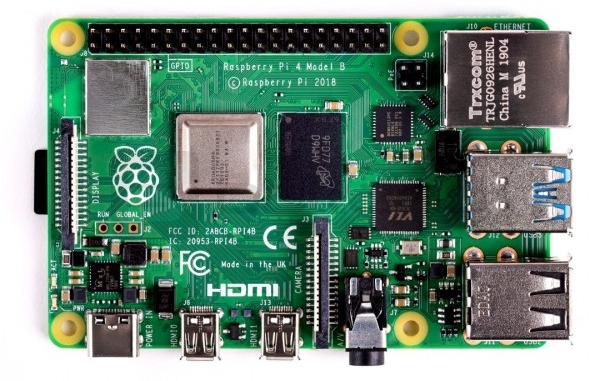
\includegraphics[width=0.5\linewidth]{raspi}
  \caption{RaspberryPi w wersji 4B\cite{raspi:img}.}
  \label{raspi:1}
\end{figure}
\clearpage
\subsection{Piny}
W RaspberryPi wyprowadzone piny odpowiedzialne są za:
\begin{itemize}[noitemsep]
  \item wyprowadzenie masy,
  \item zasilanie 3.3V i 5V,
  \item interfejs UART,
  \item interfejs I$^2$C,
  \item interfejs SPI.
\end{itemize}
Rysunek \ref{raspi:2} prezentuje jak rozmieszczone są piny odpowiedzialne za poszczególne funkcje. Piny GPIO (General Purpose IO) mogą być używane jako piny wejściowe lub wyjściowe, mogą również pełnić funkcje zegara lub stanąć się wyjściem działającym w trybie PWM.

\begin{figure}[h]
  \centering
  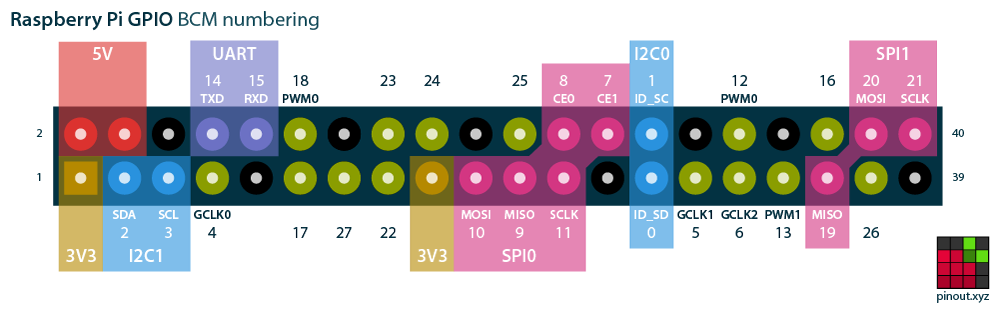
\includegraphics[width=\linewidth]{raspberry-pi-pinout}
  \caption{Piny RaspberryPi w wersji 4B\cite{pinout}.}
  \label{raspi:2}
\end{figure}

\subsection{System operacyjny}
Na RaspberryPi uruchomione mogą zostać systemy skompilowane na architekturę ARM. Najpopularniejsze z nich oparte są na Linuxie, jednym z nich jest system Raspbian\cite{raspbian}. Na RaspberryPi może uruchomiony również zostać system Windows 10 w wersji \textit{Internet of Things}\cite{w10iot}.

\section{Dioda LED}
Podstawowa obsługa diody LED polegała na włączaniu i wyłączaniu jej co sekundę. Układ został podłączony zgodnie ze schematem z rysunku \ref{sch:1}. Do zaświecenia diodą wystarczy prąd płynący przy ustawieniu stanu pinu GPIO na wysoki. Pin GPIO na wyjściu dostarcza napięcie 3.3V i może obsłużyć natężenie maksymalnie 50mA\cite{raspi:power}.

\begin{figure}[h]
  \centering
  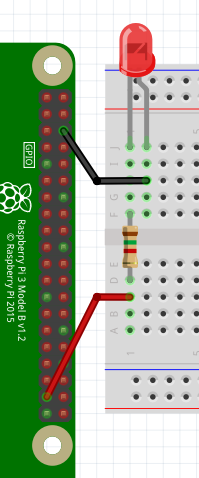
\includegraphics[height=0.4\linewidth]{sch1}
  \caption{Podłączenie diody LED.}
  \label{sch:1}
\end{figure}

\subsection{Sterowanie z poziomu powłoki systemowej}
Jądro Linuxa domyślnie wyposażone jest w sterowniki obsługujące interface GPIO. Jego cechą, tak jak wszystkich systemach operacyjnych opartych ba Unixie, jest obsługa urządzeń poprzed interface udostępniany użytkownikowi w postaci pliku. Sprowadza to obsługę urządzenia do wykonywania operacji odczytu i zapisu do określonych plików.

W przypadku obsługi diody LED w pierwszej kolejności należało aktywować odpowiedni pin w trybie wyjścia - linie 3 i 4 w listingu \ref{lst:bash}. Następnie w nieskończonej pętli skrypt zapisywał do pliku przypisanego do aktywowanego pinu wartości \lstinline{0} i \lstinline{1}. Skutkowało to zmianą napięcia na wyjściu, a w konsekwencji zapalenie i gaśnięcie diody.
%\newpage
\lstinputlisting[language=Bash, caption={Obsługa diody LED z poziomu powłoki systemowej.}, label=lst:bash]{code/led.sh}

\subsection{Sterowanie z poziomu języka Python}
Sterowanie diodą z poziomu języka Python odbywa się na podobnej zasadzie co wcześniej. Użyta biblioteka RPi.GPIO posiada API, które wewnętrznie również korzysta ze sterowników jądra systemu operacyjnego. 
\lstinputlisting[language=Python, caption={Obsługa diody LED z poziomu jezyka Python.}, label=lst:python]{code/led.py}

Wywołanie funkcji \lstinline{GPIO.setmode} odpowiada za ustawienie mapowania numeru pinu na jego fizyczny odpowiednik. Funkcja \lstinline{GPIO.setup} ustawia kierunek i początkową wartość dla pinu, a funkcja \lstinline{GPIO.output} zmienia wyjście pinu na wartość z argumentu.
\newpage
\subsection{Sterowanie przyciskiem}
Cośtam blabla
\begin{figure}[h]
  \centering
  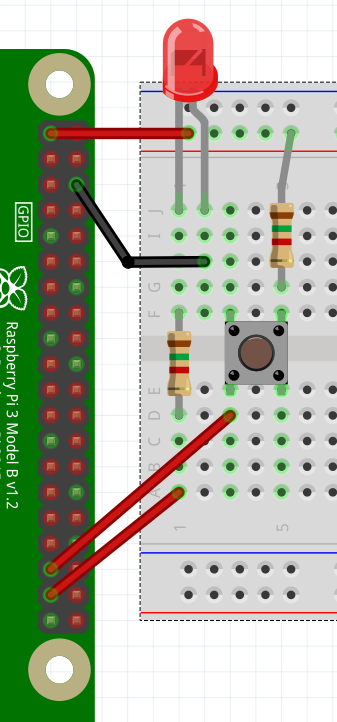
\includegraphics[height=0.4\linewidth]{sch2}
  \caption{Podłączenie diody LED i przycisku.}
  \label{sch:1}
\end{figure}

\lstinputlisting[language=Python, caption={Sterowanie diodą LED za pomocą przycisku. Najważniejsze fragmenty.}, label=lst:button, linerange={8-24}]{code/led_button.py}


\section{Pomiar temperatury}

\section{Pomiar odległości}

\section{Podsumowanie}


\newpage
\begin{thebibliography}{9}
  \bibitem{raspi}
  RaspberryPi: \url{https://pl.wikipedia.org/wiki/Raspberry_Pi}
  \bibitem{arm}
  ARM: \url{https://pl.wikipedia.org/wiki/Architektura_ARM}
  \bibitem{raspi:img}
  RaspberryPi - wygląd: \url{https://botland.com.pl/59269-thickbox_default/raspberry-pi-4-model-b-wifi-dualband-bluetooth-4gb-ram-15ghz.jpg}
  \bibitem{pinout}
  Pinout: \url{http://pinout.xyz}
  \bibitem{raspbian}
  Raspbian: https://www.raspbian.org/
  \bibitem{w10iot}
  Windows 10 IoT: \url{https://docs.microsoft.com/pl-pl/windows/iot-core/}
  \bibitem{raspi:power}
  Power pins: \url{https://elinux.org/RPi_Low-level_peripherals#Power_pins}
\end{thebibliography}
\end{document}